\documentclass[a4paper,11pt]{article}
\usepackage{amsmath,amsthm,amsfonts,amssymb,amscd,amstext,vmargin,graphics,graphicx,tabularx,multicol} 
\usepackage[francais]{babel}
\usepackage[utf8]{inputenc}  
\usepackage[T1]{fontenc} 
\usepackage{pstricks-add,tikz,tkz-tab,variations}
\usepackage[autolanguage,np]{numprint} 

\setmarginsrb{1.5cm}{0.5cm}{1cm}{0.5cm}{0cm}{0cm}{0cm}{0cm} %Gauche, haut, droite, haut
\newcounter{numexo}
\newcommand{\exo}[1]{\stepcounter{numexo}\noindent{\bf Exercice~\thenumexo} : \marginpar{\hfill /#1}}
\reversemarginpar


\newcounter{enumtabi}
\newcounter{enumtaba}
\newcommand{\q}{\stepcounter{enumtabi} \theenumtabi.  }
\newcommand{\qa}{\stepcounter{enumtaba} (\alph{enumtaba}) }
\newcommand{\initq}{\setcounter{enumtabi}{0}}
\newcommand{\initqa}{\setcounter{enumtaba}{0}}

\newcommand{\be}{\begin{enumerate}}
\newcommand{\ee}{\end{enumerate}}
\newcommand{\bi}{\begin{itemize}}
\newcommand{\ei}{\end{itemize}}
\newcommand{\bp}{\begin{pspicture*}}
\newcommand{\ep}{\end{pspicture*}}
\newcommand{\bt}{\begin{tabular}}
\newcommand{\et}{\end{tabular}}
\renewcommand{\tabularxcolumn}[1]{>{\centering}m{#1}} %(colonne m{} centrée, au lieu de p par défault) 
\newcommand{\tnl}{\tabularnewline}

\newcommand{\bmul}[1]{\begin{multicols}{#1}}
\newcommand{\emul}{\end{multicols}}

\newcommand{\trait}{\noindent \rule{\linewidth}{0.2mm}}
\newcommand{\hs}[1]{\hspace{#1}}
\newcommand{\vs}[1]{\vspace{#1}}

\newcommand{\N}{\mathbb{N}}
\newcommand{\Z}{\mathbb{Z}}
\newcommand{\R}{\mathbb{R}}
\newcommand{\C}{\mathbb{C}}
\newcommand{\Dcal}{\mathcal{D}}
\newcommand{\Ccal}{\mathcal{C}}
\newcommand{\mc}{\mathcal}

\newcommand{\vect}[1]{\overrightarrow{#1}}
\newcommand{\ds}{\displaystyle}
\newcommand{\eq}{\quad \Leftrightarrow \quad}
\newcommand{\vecti}{\vec{\imath}}
\newcommand{\vectj}{\vec{\jmath}}
\newcommand{\Oij}{(O;\vec{\imath}, \vec{\jmath})}
\newcommand{\OIJ}{(O;I,J)}


\newcommand{\reponse}[1][1]{%
\multido{}{#1}{\makebox[\linewidth]{\rule[0pt]{0pt}{20pt}\dotfill}
}}

\newcommand{\titre}[5] 
% #1: titre #2: haut gauche #3: bas gauche #4: haut droite #5: bas droite
{
\noindent #2 \hfill #4 \\
#3 \hfill #5

\vspace{-1.6cm}

\begin{center}\rule{6cm}{0.5mm}\end{center}
\vspace{0.2cm}
\begin{center}{\large{\textbf{#1}}}\end{center}
\begin{center}\rule{6cm}{0.5mm}\end{center}
}



\begin{document}
\pagestyle{empty}
\titre{Interrogation: Divisions décimales et fractions}{Nom :}{Prénom :}{Classe}{Date}


\exo{2} Poser et effectuer les opérations suivantes :
\bmul{2}

a) 85 : 6


\columnbreak


b) 10 : 11

\emul

\vspace*{4cm}

\exo{1} Pauline a effectué les divisions décimales suivantes mais elle a oublié de placer la virgule au quotient. Aide-la en ajoutant chaque virgule manquante.

\begin{center}
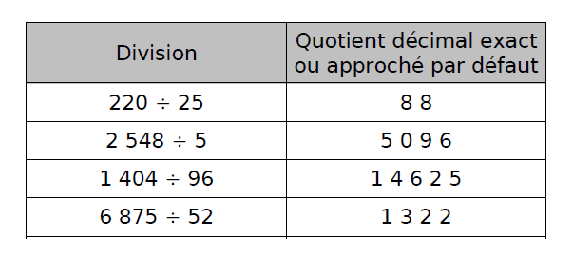
\includegraphics[scale=1]{tab.eps} 

\end{center}


\exo{2} Voici les tarifs pour le mensuel Mepmagazine :\\

- en kiosque, il coûte 99 euros pour un an (soit 12 magazines) ;\\
- en prenant un abonnement, les 12 numéros coûtent 63 euros et les 24 numéros coûtent 114 euros.\\

\q Donner le prix d'un magazine suivant qu'on l'achète ou que l'on s'y abonne pour 12 ou 24 numéros. Quelle est la solution la plus avantageuse?\\

\noindent \reponse[4]\\


\exo{1,5} Pour chaque figure, indique la fraction de la surface totale qui est colorée.

\bmul{2}

\begin{flushleft}

\includegraphics[scale=1]{fraction1.eps} 
\end{flushleft}
\reponse[1]

\columnbreak

\begin{flushleft}
\includegraphics[scale=1]{fraction2.eps} 
\end{flushleft}
\reponse[1]
\emul

\newpage

\exo{2}

\initq \q Donne une écriture fractionnaire des nombres suivants.

\bmul{4}
\qa cinq douzièmes
\reponse[1]

\columnbreak

\qa deux tiers
\reponse[1]

\columnbreak

\qa cent dix neuvièmes
\reponse[1]

\columnbreak

\qa cent dix-neuvièmes
\reponse[1]

\emul

\q Détermine la fraction dont le dénominateur est le numérateur de $\dfrac{41}{17}$ et dont le numérateur est le triple du dénominateur de $\dfrac{53}{9}$.\\
\reponse[2]\\




\exo{1,5}

\initq \q Écris, sous forme de fraction, l'abscisse de chaque point.

\includegraphics[scale=1]{demidte.eps} \\


\q Place les points suivants sur l'axe gradué : A($\dfrac{3}{6}$) ; B$(\dfrac{6}{6})$  ; C ($\dfrac{10}{6}$) et D($\dfrac{2}{3}$).\\

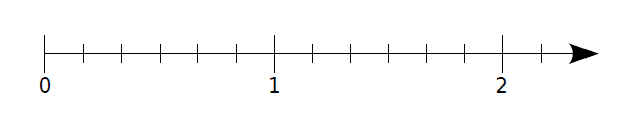
\includegraphics[scale=1]{dtes.eps} 




\end{document}
